\vspace*{4cm}
\part{Thread}\label{part:Thread}
Robin Bobst
\vspace*{\fill}
\clearpage

\section{Einleitung}\label{sec:EinleitungThread}
Thread ist ein auf IPv6 basiertes Netzwerkprotokoll, das speziell für Internet of Things (IoT) Anwendungen entwickelt wurde. Die einzelnen Teilnehmer im Netzwerk verbinden sich zu einem Mesh-Netzwerk. Wie in der Abbildung \ref{fig:ThreadProtokollLayer} ersichtlich verwendet Thread für eine effiziente Kommunikation mit IPv6-Paketen das Kommunikationsprotokoll 6LoWPAN (IPv6 over Low Power Personal Area Network). 6LoWPAN wendet ein Header-Kompressionsverfahren an, welches es ermöglicht die IPv6-Pakete über den Standard IEEE-802.15.4 zu übermitteln. Dank diesem Standard ist es machbar, die mit Thread entwickelten Geräte so energieeffizient zu gestalten, dass ein Batteriebetrieb realisierbar ist. In der Tabelle \ref{table:MerkmaleThread} sind die wichtigsten Merkmale von Thread aufgelistet. Im Juli 2014 wurde die Thread Working Group ins Leben gerufen, bei der folgende Firmen Bestandteil der Gruppe sind: Nest Labs, Samsung, ARRM Holdings, Qualcom, NXP Semiconductors, Silicon Labs, Big Ass Solutions, Somfy, OSRAM Tyco International und Yale. Ab August 2018 Apple trat auch Apple der Arbeitsgruppe bei, um das Prokoll populär zu machen. \\

\begin{figure}[H]
	\centering
	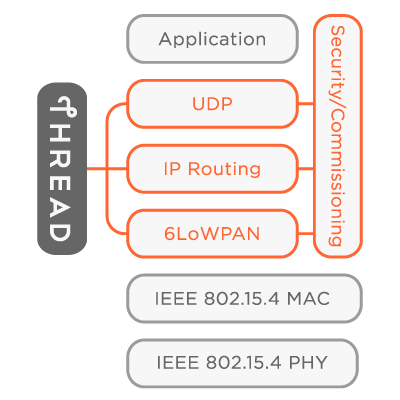
\includegraphics[width=0.5\textwidth]{threadlayerprotocols.png}
	\caption{Thread Protokoll Layer \cite{erickson_picture_2019}}
	\label{fig:ThreadProtokollLayer}
\end{figure}

\begin{table}[H]
	\centering
	\begin{adjustbox}{width=1\textwidth}
	\begin{tabular}{@{}lllll@{}}
		\cmidrule(r){1-2} \cmidrule(l){4-5}
		\multicolumn{2}{|c|}{\textbf{Netzwerk}}                                                              & \multicolumn{1}{l|}{} & \multicolumn{2}{c|}{\textbf{Applikation}}                                                                           \\ \cmidrule(r){1-2} \cmidrule(l){4-5} 
		\multicolumn{1}{|l|}{\textbf{Merkmal}}      & \multicolumn{1}{l|}{\textbf{Beschreibung}}             & \multicolumn{1}{l|}{} & \multicolumn{1}{l|}{\textbf{Merkmal}}                   & \multicolumn{1}{l|}{\textbf{Beschreibung}}                \\ \cmidrule(r){1-2} \cmidrule(l){4-5} 
		\multicolumn{1}{|l|}{IEEE 802.15.4}         & \multicolumn{1}{l|}{Protokoll}                         & \multicolumn{1}{l|}{} & \multicolumn{1}{l|}{IPv6}                               & \multicolumn{1}{l|}{IP-Kommunikation}                     \\ \cmidrule(r){1-2} \cmidrule(l){4-5} 
		\multicolumn{1}{|l|}{MAC Security}          & \multicolumn{1}{l|}{Verschlüsselte Übertragung}        & \multicolumn{1}{l|}{} & \multicolumn{1}{l|}{UDP}                                & \multicolumn{1}{l|}{UDP-Sockets}                          \\ \cmidrule(r){1-2} \cmidrule(l){4-5} 
		\multicolumn{1}{|l|}{6LoWPAN}               & \multicolumn{1}{l|}{Effiziente IPv6 Paket Übertragung} & \multicolumn{1}{l|}{} & \multicolumn{1}{l|}{CoAP}                               & \multicolumn{1}{l|}{Client und Server}                    \\ \cmidrule(r){1-2} \cmidrule(l){4-5} 
		\multicolumn{1}{|l|}{Mesh Routing}          & \multicolumn{1}{l|}{Many-to-many Kommunikation}        & \multicolumn{1}{l|}{} & \multicolumn{1}{l|}{DHCPv6}                             & \multicolumn{1}{l|}{Client und Server}                    \\ \cmidrule(r){1-2} \cmidrule(l){4-5} 
		&                                                        &                       &                                                         &                                                           \\ \cmidrule(r){1-2} \cmidrule(l){4-5} 
		\multicolumn{2}{|c|}{\textbf{Boarder Router}}                                                        & \multicolumn{1}{l|}{} & \multicolumn{2}{c|}{\textbf{Weitere Merkmale}}                                                                      \\ \cmidrule(r){1-2} \cmidrule(l){4-5} 
		\multicolumn{1}{|l|}{Web - UI}              & \multicolumn{1}{l|}{Für Netzwerk Menagement}           & \multicolumn{1}{l|}{} & \multicolumn{1}{l|}{Periodic parent search}             & \multicolumn{1}{l|}{Endgerät wechselt zu besserem Parent} \\ \cmidrule(r){1-2} \cmidrule(l){4-5} 
		\multicolumn{1}{|l|}{Externer Kommissioner} & \multicolumn{1}{l|}{Externes Gerät für Neuaufnahme}    & \multicolumn{1}{l|}{} & \multicolumn{1}{l|}{Jam Detection}                      & \multicolumn{1}{l|}{Signal Stau verhindern}               \\ \cmidrule(r){1-2} \cmidrule(l){4-5} 
		\multicolumn{1}{|l|}{NAT64}                 & \multicolumn{1}{l|}{Kommunikation mit IPv4}            & \multicolumn{1}{l|}{} & \multicolumn{1}{l|}{Child Supervision}                  & \multicolumn{1}{l|}{Endgerät überprüfen}                  \\ \cmidrule(r){1-2} \cmidrule(l){4-5} 
		\multicolumn{1}{|l|}{wpantund}              & \multicolumn{1}{l|}{Interface Treiber}                 & \multicolumn{1}{l|}{} & \multicolumn{1}{l|}{Inform previous parent on reattach} & \multicolumn{1}{l|}{Endgerät Menagement}                  \\ \cmidrule(r){1-2} \cmidrule(l){4-5} 
	\end{tabular}
	\end{adjustbox}
	\caption{Merkmale Thread \cite{thread_group_what_2020}}
	\label{table:MerkmaleThread}
\end{table}

